
\begin{exercise}
	Να εφαρμοσθεί ο αλγόριθμος plot-line για τα σημεία: $ P_1(1,1),  P_2(4,13)$. Προκύπτουν συνεχόμενα pixel αν λύσω ως προς \(x\) και μεταβάλλω τα \(y\);
	
\end{exercise}

\begin{solution}
	Τα σημεία μεταξύ των οποίων θέλω να σχεδιάσω ευθεία είναι: $ P_1(1,1),  P_2(4,13)$. Επομένως:
\begin{align*}
(P_1 P_2) : y - y_1 &= \lambda (x - x_1)  \Rightarrow  
y - y_1 = \cfrac{y_2 - y_1}{x_2 - x_1} (x - x_1) \Rightarrow  \\ 
\Rightarrow y & = y_1 \cfrac{x_2 - x_1}{x_2 - x_1} + x \cfrac{y_2 - y_1}{x_2 - x_1} \Rightarrow
 y= \cfrac{ y_2 - y_1}{x_2 - x_1} \cdot x + \cfrac{x_2 y_1 - x_1 y_2}{x_2 - x_1} \Rightarrow \\
\Rightarrow y &= sx +c, \ \text{όπου} \ s = \cfrac{ y_2 - y_1}{x_2 - x_1} \ \text{και} \ c = \cfrac{x_2 y_1 - x_1 y_2}{x_2 - x_1} \tag{1}
\end{align*}	
	
Αντικαθιστώντας τις συντεταγμένες:
\[
	s = \cfrac{13-1}{4-1} = \cfrac{12}{3} = 4 > 1 \qquad \text{και} \qquad 
	c = \cfrac{4\cdot 1 - 1\cdot 13}{4-1} = -3
\]	
	
	
Συνεπώς η εξίσωση είναι $y = 4x-3$a.
Επειδή $s>1$ (κλίση μεγαλύτερη του $1$), λύνω την $\mathrm{(1)}$ ως προς $x$ και μεταβάλλω τα $y$.

Η $\mathrm{(1)}$ λυμένη ως προς $x$ γράφεται $x= \cfrac{1}{4} y + \cfrac{3}{4}$. Επειδή βγαίνουν συντεταγμένες μη ακέραιες, κάνω στρογγύλευση.
 	
\begin{itemize}
  \item $y_1 = 1 \Rightarrow (x,y) = \left( \cfrac{1}{4} \cdot 1 + \cfrac{3}{4}, 1 \right) = \left( 1, 1 \right)$
  \item $y_2 = 2 \Rightarrow (x,y) = \left( \cfrac{1}{4} \cdot 2 + \cfrac{3}{4}, 2 \right) = \left( \cfrac{5}{4}, 2 \right) = (1.25, 2) \xRightarrow{\text{rounding}} (x,y) = (1,2)$
  \item $y_3 = 3 \Rightarrow (x,y) = \left( \cfrac{1}{4} \cdot 3 + \cfrac{3}{4}, 3 \right) = \left( \cfrac{6}{4}, 3 \right) = (1.5, 3) \xRightarrow{\text{rounding}} (x,y) = (2,3)$
  \item $y_4 = 4 \Rightarrow (x,y) = \left( \cfrac{1}{4} \cdot 4 + \cfrac{3}{4}, 4 \right) = \left( \cfrac{7}{4}, 4 \right) = (1.75, 4) \xRightarrow{\text{rounding}} (x,y) = (2,4)$
  \item $y_5 = 5 \Rightarrow (x,y) = \left( \cfrac{1}{4} \cdot 5 + \cfrac{3}{4}, 5 \right) = \left( \cfrac{8}{4}, 5 \right) = (2, 5) \xRightarrow{\text{rounding}} (x,y) = (2,5)$
  \item $y_6 = 6 \Rightarrow (x,y) = \left( \cfrac{1}{4} \cdot 6 + \cfrac{3}{4}, 6 \right) = \left( \cfrac{9}{4}, 6 \right) = (2.25, 6) \xRightarrow{\text{rounding}} (x,y) = (2,6)$
  \item $y_7 = 7 \Rightarrow (x,y) = \left( \cfrac{1}{4} \cdot 7 + \cfrac{3}{4}, 7 \right) = \left( \cfrac{10}{4}, 7 \right) = (2.5, 7) \xRightarrow{\text{rounding}} (x,y) = (3,7)$
  \item $y_8 = 8 \Rightarrow (x,y) = \left( \cfrac{1}{4} \cdot 8 + \cfrac{3}{4}, 8 \right) = \left( \cfrac{11}{4}, 8 \right) = (2.75, 8) \xRightarrow{\text{rounding}} (x,y) = (3,8)$
  \item $y_9 = 9 \Rightarrow (x,y) = \left( \cfrac{1}{4} \cdot 9 + \cfrac{3}{4}, 9 \right) = \left( \cfrac{12}{4}, 9 \right) = (3, 9) \xRightarrow{\text{rounding}} (x,y) = (3,9)$
  \item $y_{10} = 10 \Rightarrow (x,y) = \left( \cfrac{1}{4} \cdot 10 + \cfrac{3}{4}, 10 \right) = \left( \cfrac{13}{4}, 10 \right) = (3.25, 10) \xRightarrow{\text{rounding}} (x,y) = (3,10)$
  \item $y_{11} = 11 \Rightarrow (x,y) = \left( \cfrac{1}{4} \cdot 11 + \cfrac{3}{4}, 11 \right) = \left( \cfrac{14}{4}, 11 \right) = (3.5, 11) \xRightarrow{\text{rounding}} (x,y) = (4,11)$
  \item $y_{12} = 12 \Rightarrow (x,y) = \left( \cfrac{1}{4} \cdot 12 + \cfrac{3}{4}, 12 \right) = \left( \cfrac{15}{4}, 12 \right) = (3.75, 12) \xRightarrow{\text{rounding}} (x,y) = (4,12)$
  \item $y_{13} = 13 \Rightarrow (x,y) = \left( \cfrac{1}{4} \cdot 13 + \cfrac{3}{4}, 13 \right) = \left( \cfrac{16}{4}, 13 \right) = (4, 13) \xRightarrow{\text{rounding}} (x,y) = (4,13)$
\end{itemize}

Παρατηρούμε όπως ήταν προβλεπόμενο, ότι φωτίζονται συνεχόμενα pixel.

\begin{figure}[hbt]
	\begin{center}
		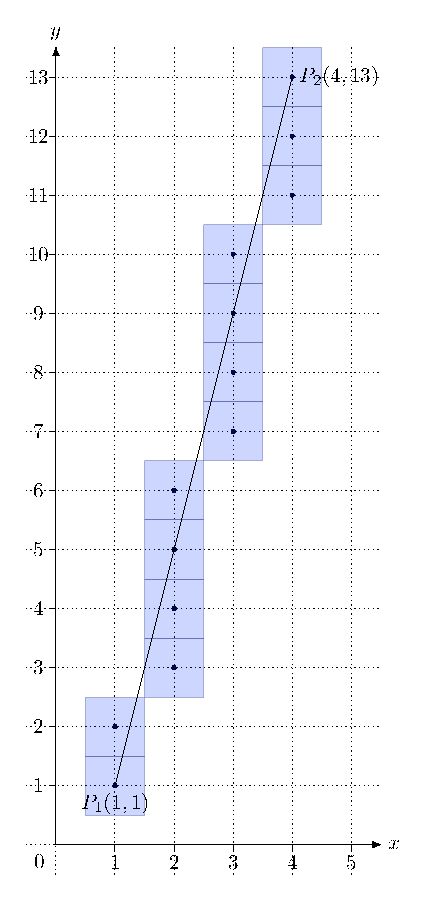
\includegraphics[scale=0.8]{Chapter1/Exercises/ex1-graph.pdf}
	\end{center}
\caption{Γραφική λύση άσκησης}
\end{figure}

\end{solution}